%========================================
%              Chapter              
%======================================== 
\chapter{Figure and Table Chapter}
\lipsum[5]
%========================================
%              Section               
%======================================== 
\section{Figures}

The ``\verb|figure|'' environment should be used for figures. One or
more images can be placed within a figure. If your figure contains
third-party material, you must clearly identify it as such, as shown
in the example below.
\begin{figure}[h]
	\centering
	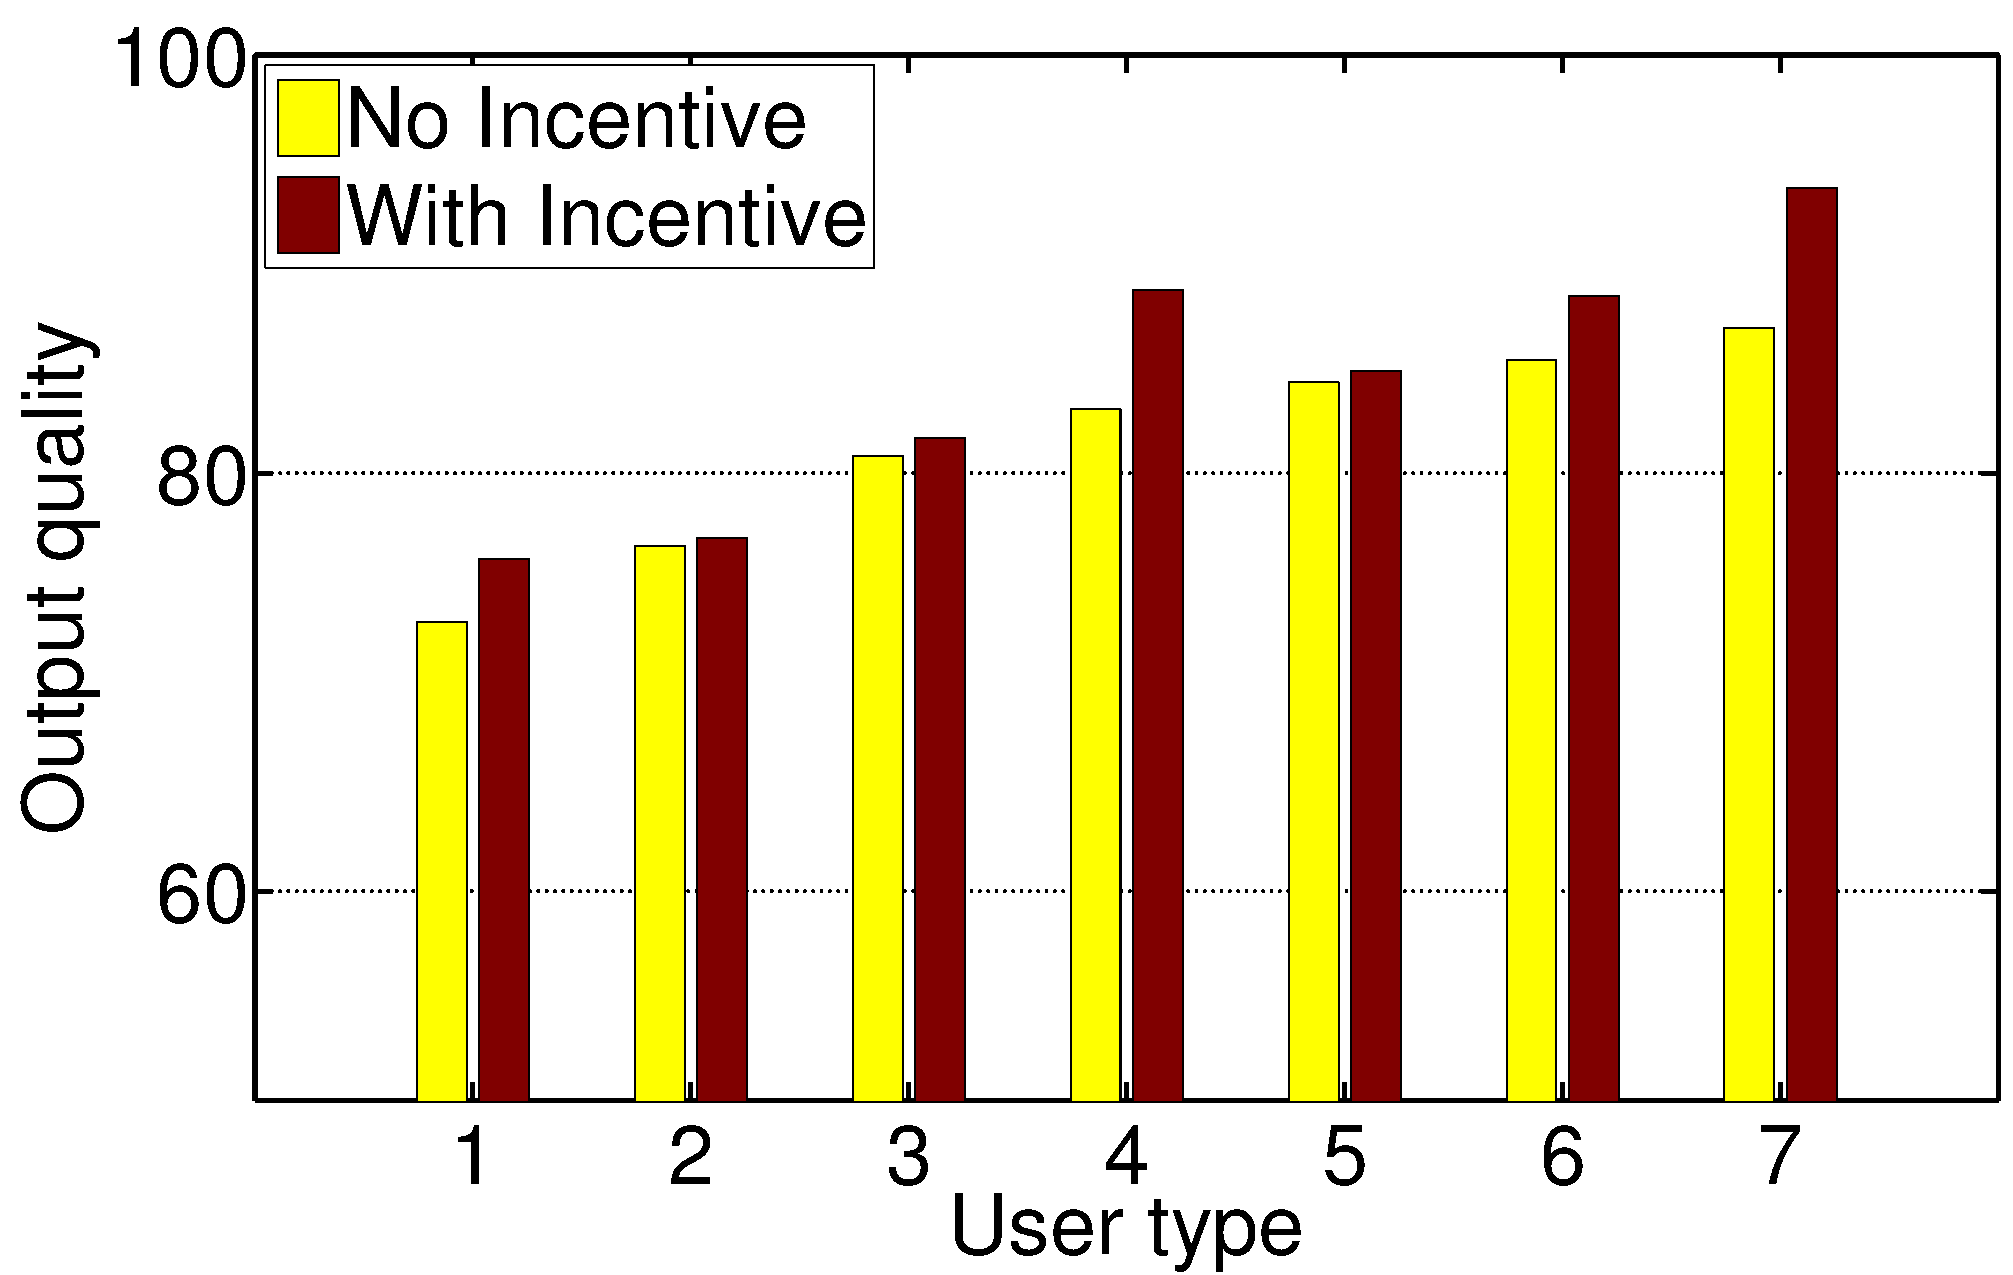
\includegraphics[width=\linewidth]{fig1}
	\caption{The figure with long long long long long long long long long long long long long long long long long long long long long long long long long long long long long long long long caption and links. (\url{https://goo.gl/VLCRBB}).}
\end{figure}



\lipsum[1-2]
\begin{landscape} % Require pdflscape and everypage packadge
	\begin{figure}[h]
		\centering
		% will generate blank page if use full  \linewidth
		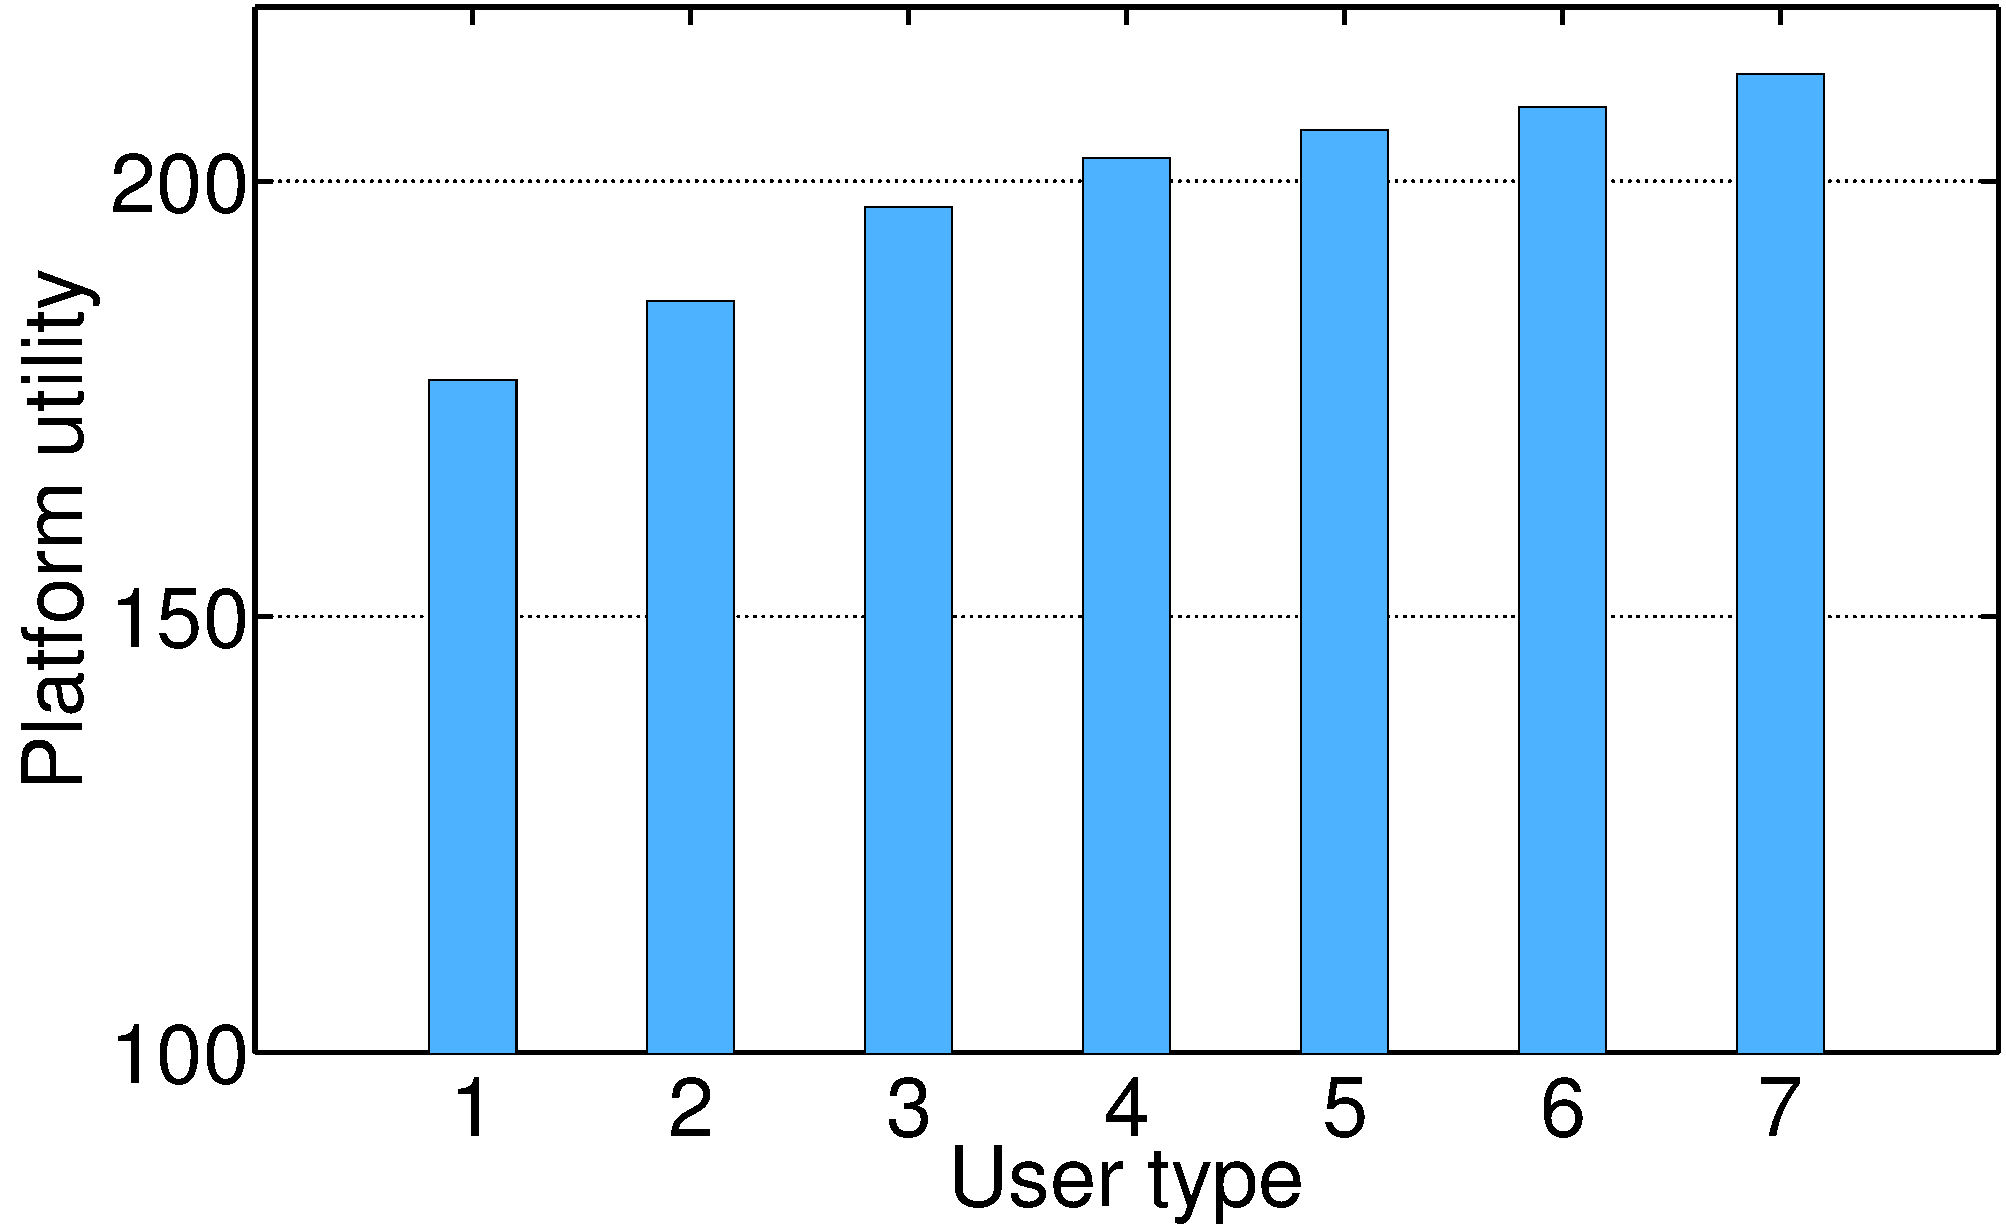
\includegraphics[width=.9\linewidth]{fig3} 
		\caption{Continues figures in landscape mode. (first)}
	\end{figure}

	\begin{figure}[h]
	\centering
	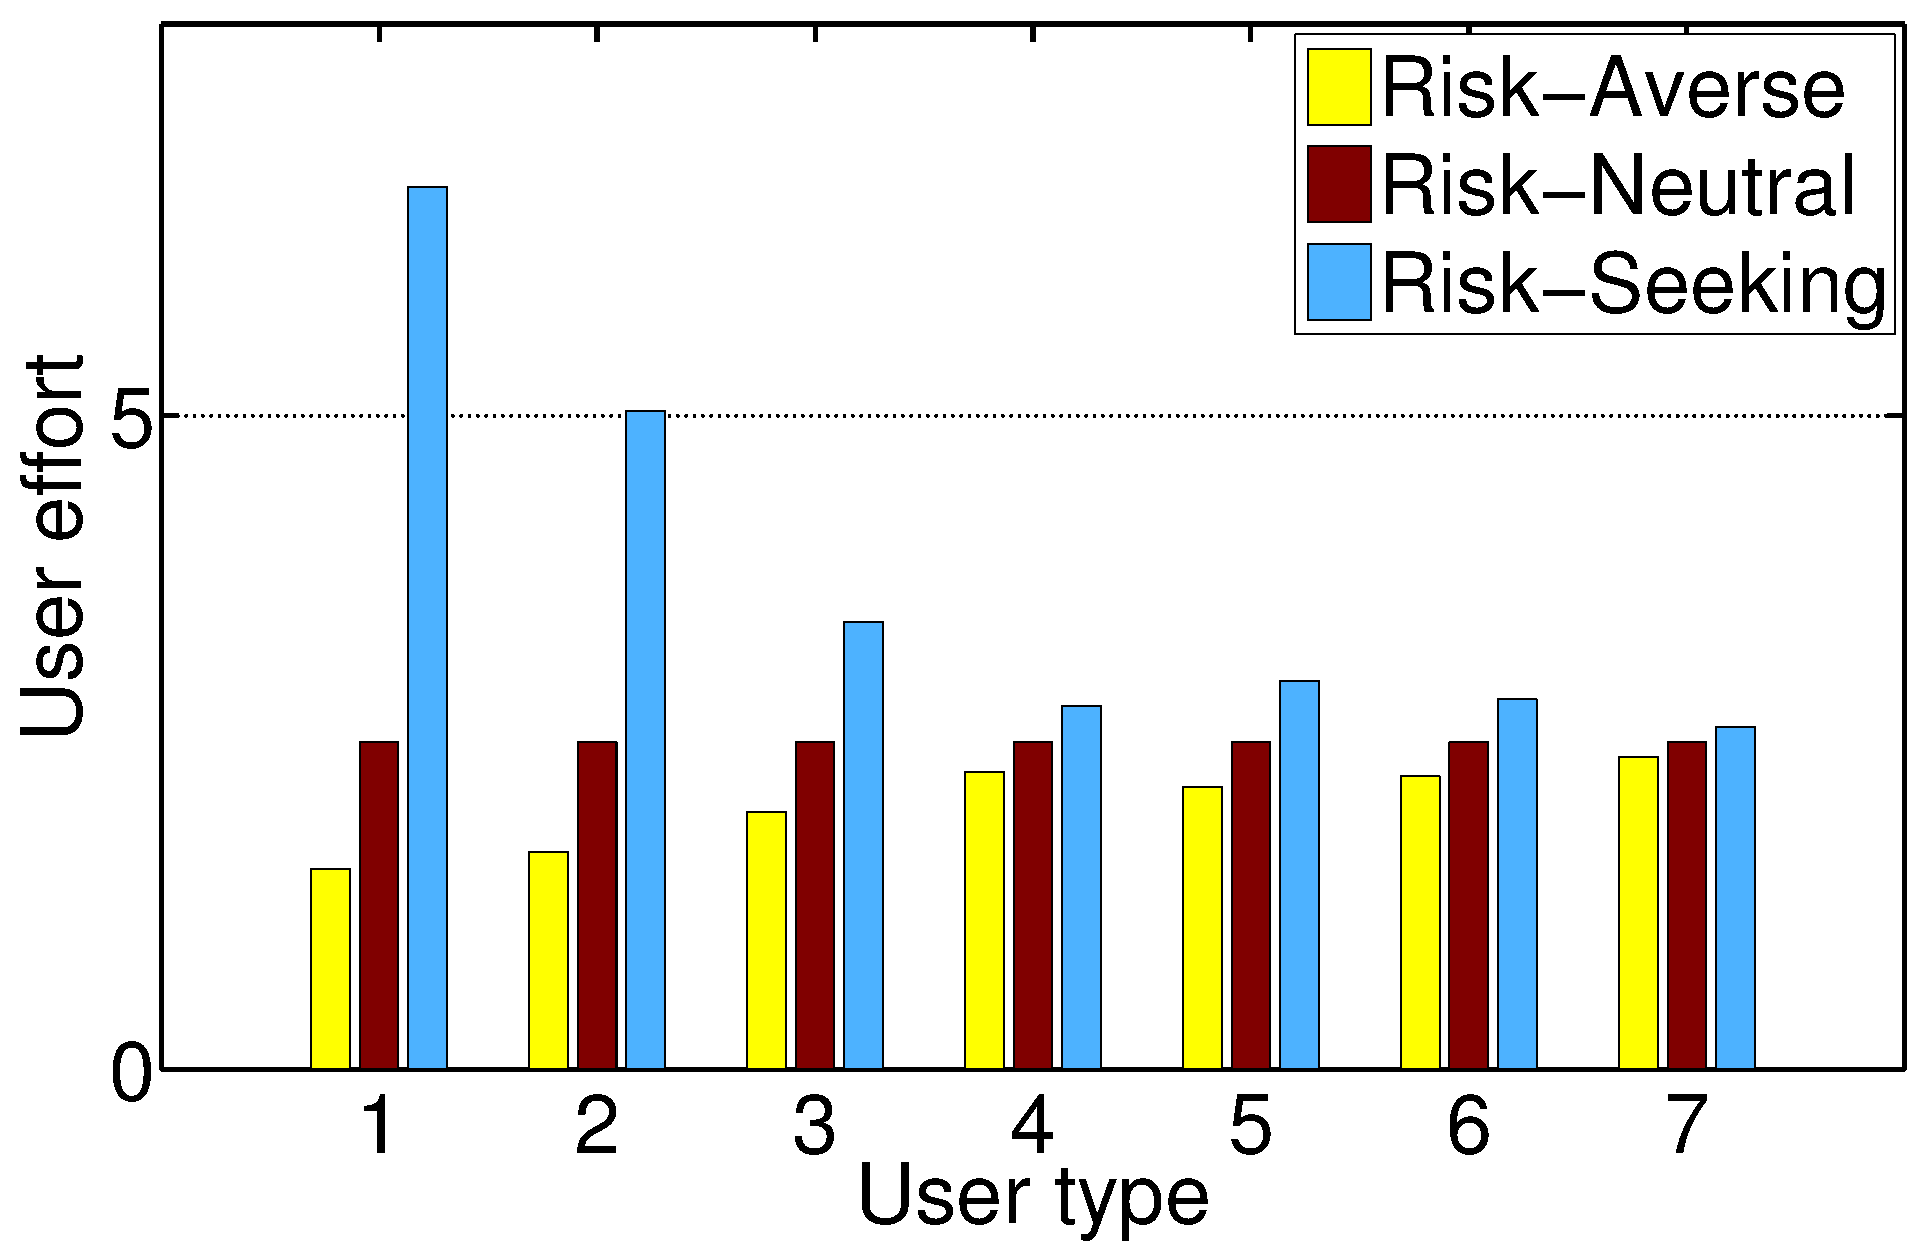
\includegraphics[width=\linewidth]{fig4}
	\caption{Continues figures in landscape mode. (second)}
	\end{figure}
\end{landscape}

Your figures should contain a caption which describes the figure to
the reader. Figure captions go below the figure. Your figures should
{\bfseries also} include a description suitable for screen readers, to
assist the visually-challenged to better understand your work.

Figure captions are placed {\itshape below} the figure.


\begin{landscape} % Require pdflscape and everypage packadge
	\begin{figure}[h]
		\centering
		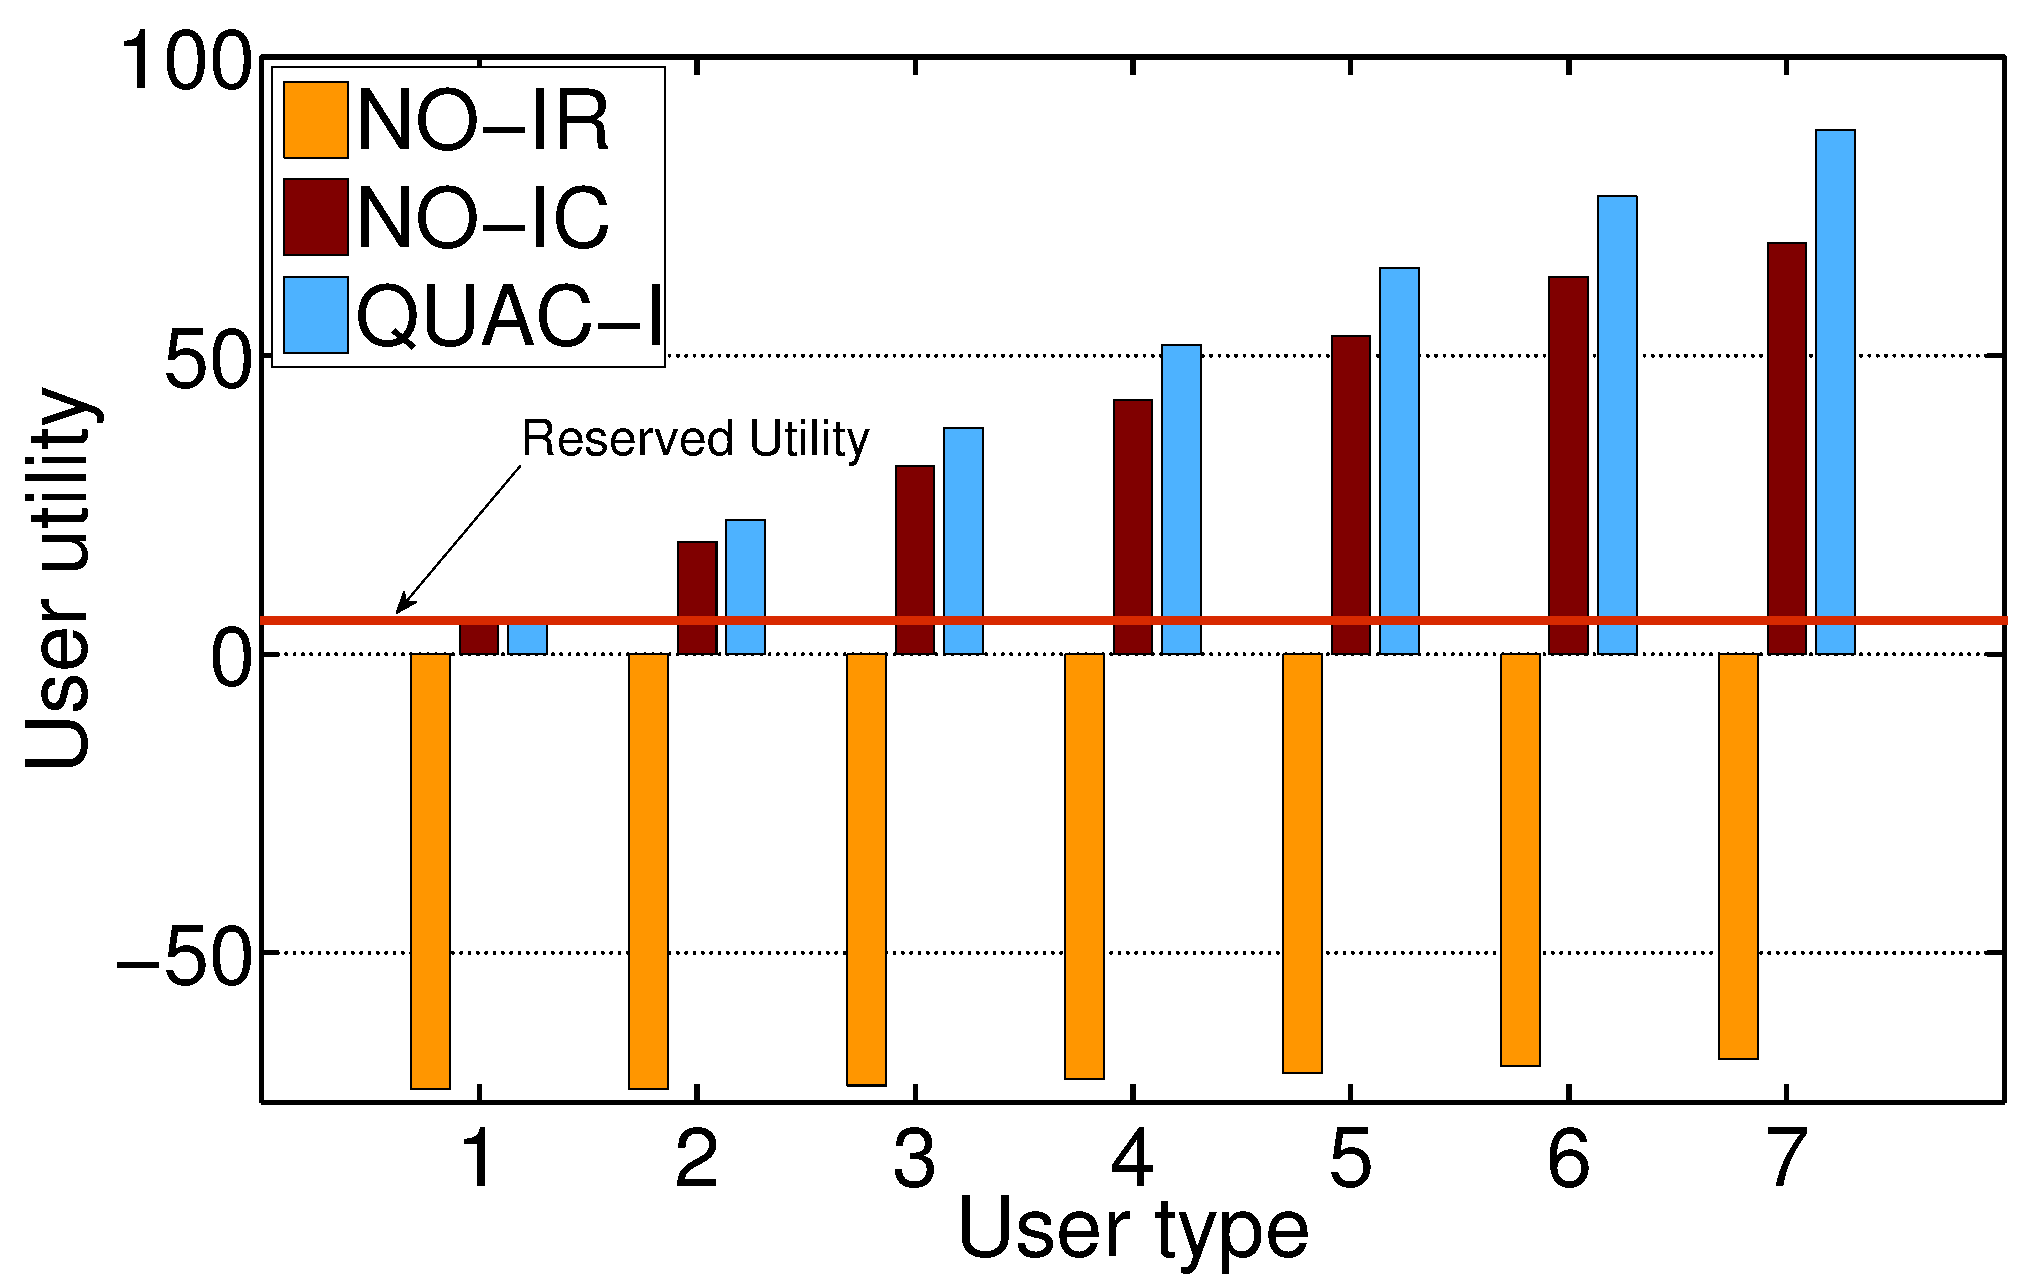
\includegraphics[width=.9\linewidth]{fig6}
		\caption{Example of a figure in landscape mode. Use \texttt{$\backslash$centering} to center the image}
	\end{figure}
\end{landscape}



\begin{figure}[h]
	\centering
	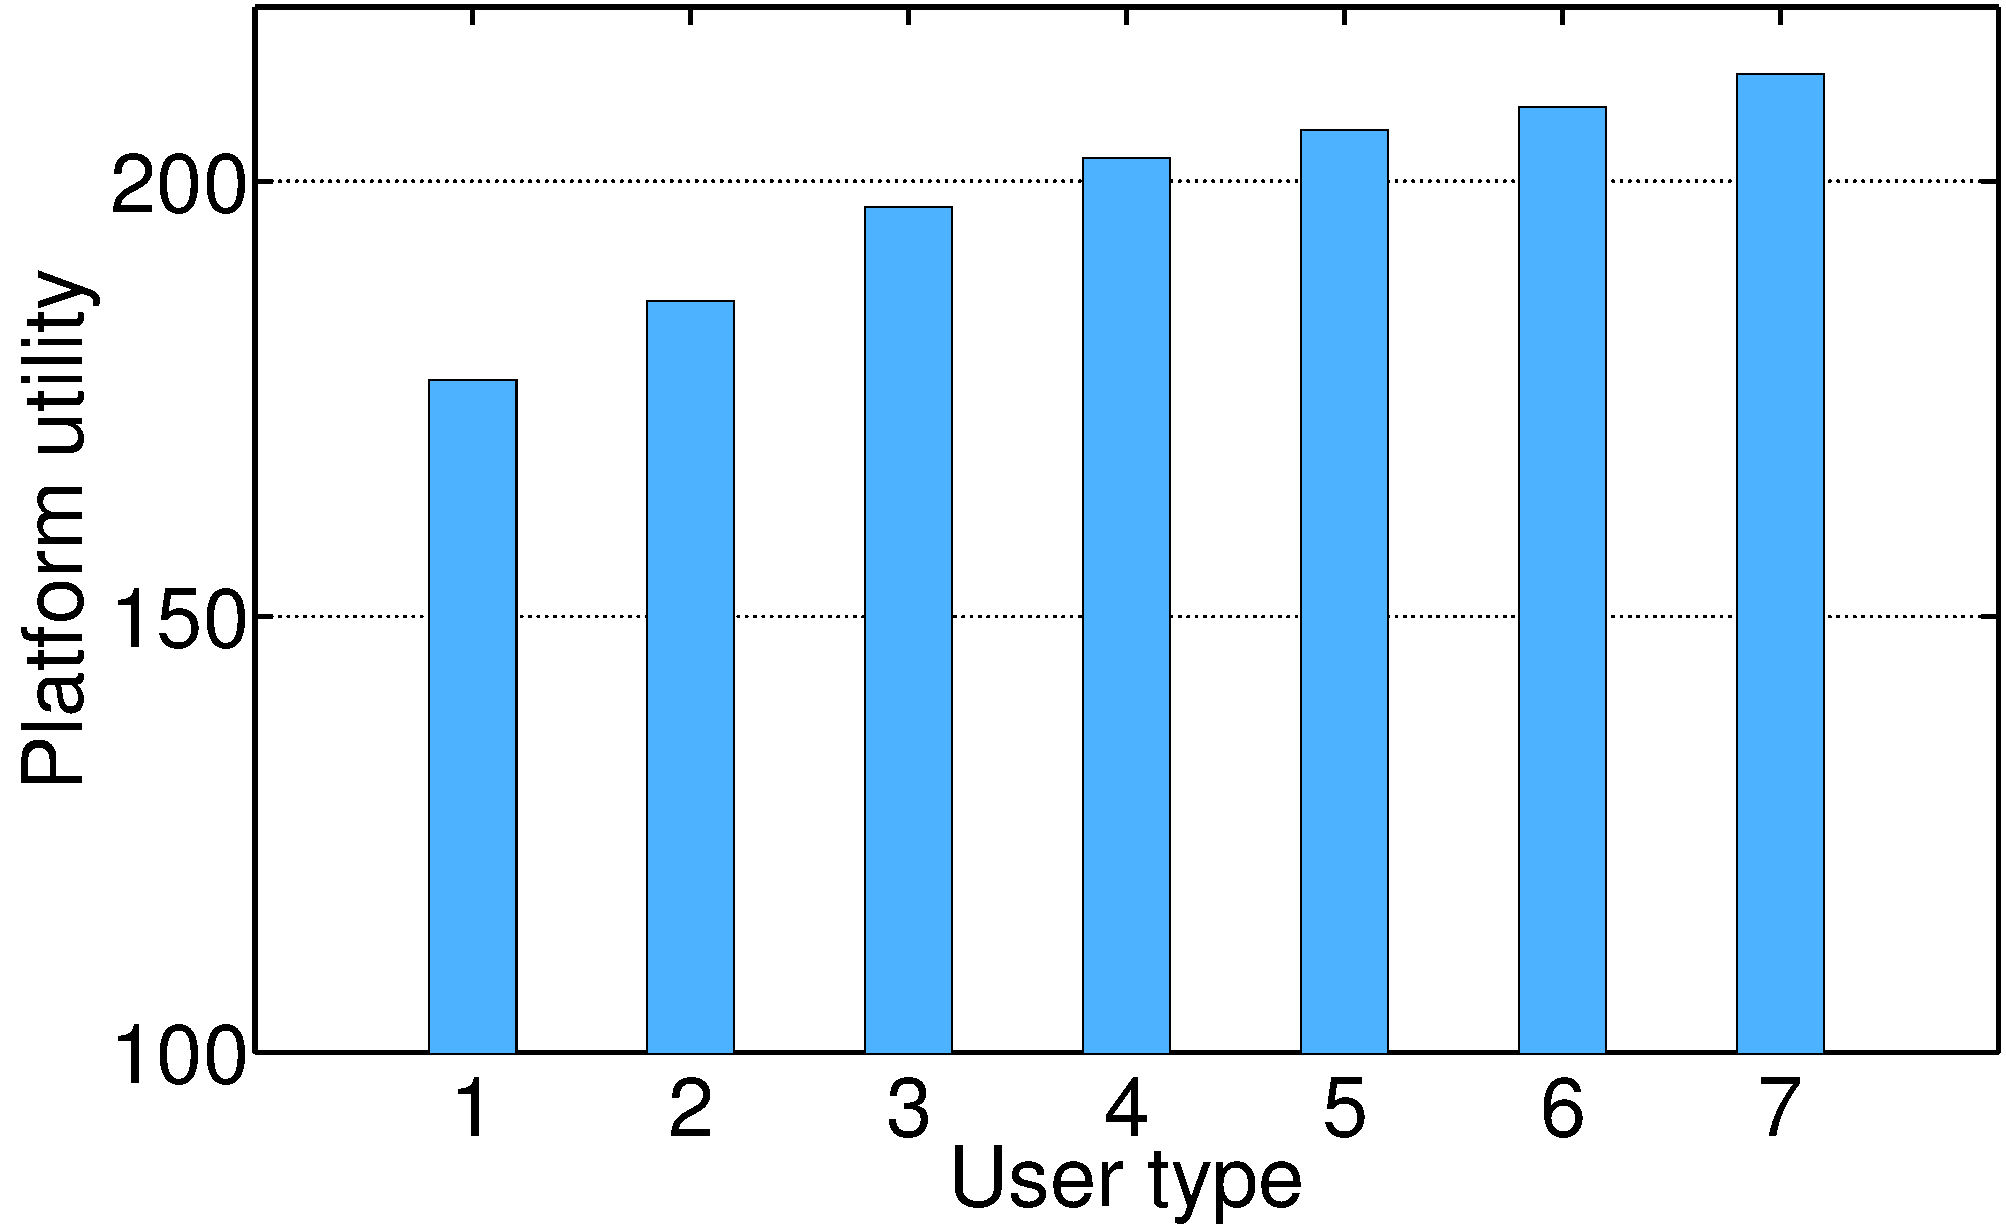
\includegraphics[width=\linewidth]{fig3}
	\caption[Short version caption for LoF, the original caption is really long]{The original realy long long long long long long long long long long long long long long long long long long long long long long long long long long long long long long figure caption.}
\end{figure}
%========================================
%              Section               
%======================================== 
\section{Tables}

The ``\verb|minesthesis|'' document class includes the ``\verb|booktabs|''
package --- \url{https://ctan.org/pkg/booktabs} --- for preparing
high-quality tables.

Table captions are placed {\itshape above} the table.

Because tables cannot be split across pages, the best placement for
them is typically the top of the page nearest their initial cite. To
ensure this proper ``floating'' placement of tables, use the
environment \textbf{table} to enclose the table's contents and the
table caption. The contents of the table itself must go in the
\textbf{tabular} environment, to be aligned properly in rows and
columns, with the desired horizontal and vertical rules. Again,
detailed instructions on \textbf{tabular} material are found in the
\textit{\LaTeX\ User's Guide}.

Immediately following this sentence is the point at which
Table~\ref{tab:freq} is included in the input file; compare the
placement of the table here with the table in the printed output of
this document.

\begin{table}[h]
	\caption{Frequency of Special Characters}
	\label{tab:freq}
	\centering
	\begin{tabular}{ccl}
		\toprule
		Non-English or Math & Frequency   & Comments          \\
		\midrule
		\O                  & 1 in 1,000  & For Swedish names \\
		$\pi$               & 1 in 5      & Common in math    \\
		\$                  & 4 in 5      & Used in business  \\
		$\Psi^2_1$          & 1 in 40,000 & Unexplained usage \\
		\bottomrule
	\end{tabular}
\end{table}


\begin{table*}[h]
	\caption{Some Typical Commands}
	\label{tab:commands}
	\centering
	\begin{tabular}{cclccr}
		\toprule
		Command                    & A Number & Comments         & Command                    & A Number & Comments         \\
		\midrule
		\texttt{{\char'134}author} & 100      & Author           & \texttt{{\char'134}author} & 100      & Author           \\
		\texttt{{\char'134}table}  & 300      & For tables       & \texttt{{\char'134}table}  & 300      & For tables       \\
		\texttt{{\char'134}table*} & 400      & For wider tables & \texttt{{\char'134}table*} & 400      & For wider tables \\
		\bottomrule
	\end{tabular}
\end{table*}

\begin{table*}[h]
	\caption{Some Typical Commands with borders}
	\label{tab:commandswithborders}
	\begin{tabular}{|ccl|ccr|} % use | to add vertical lines
		\hline % use hline instead of toprule/midrule/bottomrule
		Command                    & A Number & Comments         & Command                    & A Number & Comments         \\
		\hline
		\texttt{{\char'134}author} & 100      & Author           & \texttt{{\char'134}author} & 100      & Author           \\
		\texttt{{\char'134}table}  & 300      & For tables       & \texttt{{\char'134}table}  & 300      & For tables       \\
		\texttt{{\char'134}table*} & 400      & For wider tables & \texttt{{\char'134}table*} & 400      & For wider tables \\
		\hline
	\end{tabular}
\end{table*}

\begin{table}[h]
	\caption{Some Typical Commands with borders}
	\label{tab:tabularexample}
	\centering
	\begin{tabular}{>{\ttfamily}m{0.1\textwidth}m{0.2\textwidth}m{0.2\textwidth}} % use | to add vertical lines
		\hline % use hline instead of toprule/midrule/bottomrule
		Command          & A Number & Comments\\
		\hline
		{\char'134}author & 100      & Author            \\
		{\char'134}table & 300      & For tables        \\
		{\char'134}table* & 400      & For wider tables \\
		{\char'134}author & 100      & Author            \\
		{\char'134}table & 300      & For tables        \\
		{\char'134}table* & 400      & For wider tables \\
		\hline
	\end{tabular}
\end{table}



To set a wider table, which takes up the whole width of the page's
live area, use the environment \textbf{table*} to enclose the table's
contents and the table caption. As with a single-column table, this
wide table will ``float'' to a location deemed more
desirable. Immediately following this sentence is the point at which
Table~\ref{tab:commands} is included in the input file; again, it is
instructive to compare the placement of the table here with the table
in the printed output of this document.
\begin{table}[h]
	\caption{Some table with really long long long long long long long long long long long long long long long long long long long long long long long long long long long long long long long long long long long caption}
	\label{tab:commandsnostar}
	\centering
	\begin{tabular}{cclccr}
		\toprule
		Command & A Number & Comments & Command  & A Number & Comments         \\
		\midrule
		\texttt{{\char'134}author} & 100      & Author           & \texttt{{\char'134}author} & 100      & Author           \\
		\texttt{{\char'134}table}  & 300      & For tables       & \texttt{{\char'134}table}  & 300      & For tables       \\
		\texttt{{\char'134}table*} & 400      & For wider tables & \texttt{{\char'134}table*} & 400      & For wider tables \\
		\bottomrule
	\end{tabular}
\end{table}



\begin{landscape}
	\begin{table}[h]
		\caption{A table in landscape mode}
		\label{tab:landscape}
%		\centering
		\begin{tabular}{cclccrlcr}
			\toprule
			Command                    & A Number & Comments         & Command                    & A Number & Comments         & Command                    & A Number & Comments         \\
			\midrule
			\texttt{{\char'134}author} & 100      & Author           & \texttt{{\char'134}author} & 100      & Author           & \texttt{{\char'134}author} & 100      & Author           \\
			\texttt{{\char'134}table}  & 300      & For tables       & \texttt{{\char'134}table}  & 300      & For tables       & \texttt{{\char'134}table}  & 300      & For tables       \\
			\texttt{{\char'134}table*} & 400      & For wider tables & \texttt{{\char'134}table*} & 400      & For wider tables & \texttt{{\char'134}table*} & 400      & For wider tables \\
			\texttt{{\char'134}author} & 100      & Author           & \texttt{{\char'134}author} & 100      & Author           & \texttt{{\char'134}author} & 100      & Author           \\
			\texttt{{\char'134}table}  & 300      & For tables       & \texttt{{\char'134}table}  & 300      & For tables       & \texttt{{\char'134}table}  & 300      & For tables       \\
			\texttt{{\char'134}table*} & 400      & For wider tables & \texttt{{\char'134}table*} & 400      & For wider tables & \texttt{{\char'134}table*} & 400      & For wider tables \\
			\texttt{{\char'134}author} & 100      & Author           & \texttt{{\char'134}author} & 100      & Author           & \texttt{{\char'134}author} & 100      & Author           \\
			\texttt{{\char'134}table}  & 300      & For tables       & \texttt{{\char'134}table}  & 300      & For tables       & \texttt{{\char'134}table}  & 300      & For tables       \\
			\texttt{{\char'134}table*} & 400      & For wider tables & \texttt{{\char'134}table*} & 400      & For wider tables & \texttt{{\char'134}table*} & 400      & For wider tables \\
			\texttt{{\char'134}author} & 100      & Author           & \texttt{{\char'134}author} & 100      & Author           & \texttt{{\char'134}author} & 100      & Author           \\
			\texttt{{\char'134}table}  & 300      & For tables       & \texttt{{\char'134}table}  & 300      & For tables       & \texttt{{\char'134}table}  & 300      & For tables       \\
			\texttt{{\char'134}table*} & 400      & For wider tables & \texttt{{\char'134}table*} & 400      & For wider tables & \texttt{{\char'134}table*} & 400      & For wider tables \\
			\bottomrule
		\end{tabular}
	\end{table}
\end{landscape}


